%%%%%%%%%%%%%%%%%%%%%%%%%%%%%%%%%%%%%%%%%%%%%%%%%%%%%%%%%%%%%%%%%%%%%%%%%%%%%%%%
%% Title (en): Multiagent Systems and Organizations                           %%
%% Title (cs): Multiagentní systémy a organizace                              %%
%%                                                                            %%
%% Author: Bc. Lukáš Kúdela                                                   %%
%% Supervisor: Prof. RNDr. Petr Štěpánek, DrSc.                               %%
%%                                                                            %%
%% Academic year: 2011/2012                                                   %%
%%%%%%%%%%%%%%%%%%%%%%%%%%%%%%%%%%%%%%%%%%%%%%%%%%%%%%%%%%%%%%%%%%%%%%%%%%%%%%%%

%%%%%%%%%%%%%%%%%%%%%%%%%%%%%%%%%%%%%%%%%%%%%%%%%%%%%%%%%%%%%%%%%%%%%%%%%%%%%%%%
\section{Example 2: Expression Evaluation}
%%%%%%%%%%%%%%%%%%%%%%%%%%%%%%%%%%%%%%%%%%%%%%%%%%%%%%%%%%%%%%%%%%%%%%%%%%%%%%%%

% Expression evaluation organziation
This example demonstrates a not-so-simple organization - the expression evaluation.
% Function invocation organization - purpose
The purpose of this organization is to facilitate divide-and-conquer expression evaluation by grouping five agents: one agent breaks the expression down (the `divide' part) and the other four compute addition, subtraction, multiplication and division (the `conquer' part).
% Assumptions
In this example, agents evaluate simple arithmetic expressions (consists of natural numbers, four binary operations - addition, subtraction, multiplication and integral division - and parentheses), but it should be apparent that any arithmetic expressions could be evaluated this way.

%%%%%%%%%%%%%%%%%%%%%%%%%%%%%%%%%%%%%%%%%%%%%%%%%%%%%%%%%%%%%%%%%%%%%%%%%%%%%%%%
\subsection*{Specification}

%%%%%%%%%%%%%%%%%%%%%%%%%%%%%%%%%%%%%%%%%%%%%%%%%%%%%%%%%%%%%%%%%%%%%%%%%%%%%%%%
\subsubsection*{Organization Part}

% 'Evaluate expression' organizaiton type
The \textit{Evaluate expression} organization type (modelled by the \texttt{EvaluateExpression\_Organization} agent class) contains five roles - \textit{Evaluator}, \textit{Adder}, \textit{Subtractor}, \textit{Multiplier} and \textit{Divider} - and two protocols - \textit{Evaluate expression} and \textit{Evaluate binary operation}.
% 'evalute-expression' organization
\textit{Evaluate expression} has one instance in the running MAS - the \textit{evaluate-expression} organization (modelled by the \texttt{evaluateExpression\_Organization} agent instance).

% 'Evaluator' role
The \textit{Evaluator} role (modelled by the \texttt{Evaluator\_Role} class) can evaluate a simple arithmetic expression.
% 'Evaluator' role - multiplicity, competences & responsibilities
The \textit{Evaluator} role is a \textit{multiple} role
\footnote{However, only one agent plays the \textit{Evaluator} role in our example.}
.
It has one competence - \textit{Evaluate expression} - and no responsibilities.

% 'Evaluate expression' competence
The \textit{Evaluate expression} competence (modelled by the \texttt{EvaluateExpression\_Competence} class) is a competence to evaluate a simple arithmetic expression.
% 'Evaluate expression' competence - argument & result
It has one argument - an expression string - and one result - the integral value of this expression. 

% 'Adder' role
The \textit{Adder} role (modelled by the \texttt{Adder\_Role} class) can perform addition of two simple arithmetic expressions.
% 'Adder' role - multiplicity, competences & responsibilities
The \textit{Adder} role is a \textit{single} role.
It has no competences and one responsibility - \textit{Add}.

% 'Add' responsibility
The \textit{Add} responsibility (modelled by the \texttt{Add\_Responsibility} class) is a responsibility to perform addition of two integers.
% 'Add' responsibility - argument & result
It has two arguments - a pair of addends - and one result - their sum.

% 'Subtractor' role
The \textit{Subtractor} role (modelled by the \texttt{Subtractor\_Role} class) can perform subtraction of two simple arithmetic expressions.
% 'Subtractor' role - multiplicity, competences & responsibilities
The \textit{Adder} role is a \textit{single} role.
It has no competences and one responsibility - \textit{Subtract}.

% 'Subtract' responsibility
The \textit{Subtract} responsibility (modelled by the \texttt{Subtract\_Responsibility} class) is a responsibility to perform subtraction of two integers.
% 'Subtract' responsibility - argument & result
It has two arguments - a minuend and a subtrahend - and one result - their difference.

% 'Multiplier' role
The \textit{Multiplier} role (modelled by the \texttt{Multiplier\_Role} class) can perform multiplication of two simple arithmetic expressions.
% 'Multiplier' role - multiplicity, competences & responsibilities
The \textit{Adder} role is a \textit{single} role.
It has no competences and one responsibility - \textit{Multiply}.

% 'Multiply' responsibility
The \textit{Multiply} responsibility (modelled by the \texttt{Multiply\_Responsibility} class) is a responsibility to perform multiplication of two integers.
% 'Multiply' responsibility - argument & result
It has two arguments - a pair of factors - and one result - their product.

% 'Divider' role
The \textit{Divider} role (modelled by the \texttt{Divider\_Role} class) can perform division of two simple arithmetic expressions.
% 'Divider' role - multiplicity, competences & responsibilities
The \textit{Divider} role is a \textit{single} role.
It has no competences and one responsibility - \textit{Divide}. 

% 'Divide' responsibility
The \textit{Divide} responsibility (modelled by the \texttt{Divide\_Responsibility} class) is a responsibility to perform integral division of two integers.
% 'Multiply' responsibility - argument & result
It has two arguments - a dividend and a divisor - and one result - their quotient.

% 'Binary operator' role
In the following, we will use the \textit{Binary operator} abstract role to refer to refer to the \textit{Adder}, \textit{Subtractor}, \textit{Multiplier} or \textit{Divisor} role where it is not necessary to distinguish between them.

%%%%%%%%%%%%%%%%%%%%%%%%%%%%%%%%%%%%%%%%%%%%%%%%%%%%%%%%%%%%%%%%%%%%%%%%%%%%%%%%
\subsubsection*{Protocol Part}

% 'Evaluate expresion' protocol
The \textit{Evaluate expression} protocol (modelled by the \texttt{EvaluateExpressionProtocol} class) is a protocol through which an \textit{Binary operator} (the initiator party, modelled by the \texttt{EvaluateExpression\_InitiatorParty}) requests an \textit{Evaluator} (the responder party, modelled by the \texttt{EvaluateExpression\_RespodnerParty}) to evaluate an expression.

% 'Evaluate expression request' message
The \textit{Evaluate expression request} message (modelled by the \texttt{EvaluateExpressionReqestMessage} class) is a message sent by a \textit{Binary operator} to an \textit{Evaluator} requesting the latter to evaluate an expression.

% 'Evalaute expression reply' message
The \textit{Evaluate expression reply} message (modelled by the \texttt{EvaluateExpressionReplyMessage} class) is a message sent by an \textit{Evaluator} to a \textit{Binary operator} informing the latter about the value of the evaluated expression.

% 'Evaluate binary operation' protocol
The \textit{Evaluate binary operation} protocol (modelled by the \texttt{EvaluateBinaryOperation} class) is a protocol through which an \textit{Evaluator} (the initiator party, modelled by the \texttt{EvaluateBinaryOperation\_InitiatorParty}) requests a \textit{Binary operator} (the responder party, modelled by the \texttt{EvaluateBinaryOperation\_RespodnerParty}) to evaluate a binary operation.

% 'Evalaute binary operation request' message
The \textit{Evaluate binary operation request} message (modelled by the \texttt{EvaluateBinaryOperationReqestMessage} class) is a message sent by a \textit{Evaluator} to a \textit{Binary Operator} requesting the latter to evaluate a binary operation between two operand expressions.

% 'Evaluate binary operation reply' message
The \textit{Evaluate binary operation reply} message (modelled by the \texttt{EvaluateBinaryOperationReplyMessage} class) is a message sent by a \textit{Binary operator} to an \textit{Evaluator} informing the latter about the value of the evaluated binary operation.

%%%%%%%%%%%%%%%%%%%%%%%%%%%%%%%%%%%%%%%%%%%%%%%%%%%%%%%%%%%%%%%%%%%%%%%%%%%%%%%%
\subsubsection*{Player Part}

% 'Blank' player type
The \textit{Blank} player type (modelled by the \texttt{Blank\_Player} agent class) is a player with no capabilities.
It has one instance in the running MAS - \textit{player1}.
% 'player1' player
\textit{player1} (modelled by the \texttt{player1} agent instance) intends to enact the \textit{Evaluator} role in the \textbf{evaluate-expression} organization and to perform the role's \textit{Evaluate expression} competence - to have an expression evaluated by the players of the \textit{Binary operator} roles.

% 'Addition computer' player type
The \textit{Addition computer} player type (modelled by the \texttt{AdditionComputer\_Player} agent class) is a player capable of computing the addition operation.
It has one instance in the running MAS - \textit{player2}.
% 'player2' player
\textit{player2} (modelled by the \texttt{player2} agent instance) intends to enact the \textit{Adder} role in the \textbf{evaluate-expression} organization and perform the role's \textit{Add} responsibility - to compute addition during the evaluation of the expression from the player of the \textit{Evaluator} role.

% 'Subtraction computer' player type
The \textit{Subtraction computer} player type (modelled by the \texttt{SubtractionComputer\_Player} agent class) is a player capable of computing the subtraction operation.
It has one instance in the running MAS - \textit{player3}.
% 'player3' player
The intention of \textit{player3} (modelled by the \texttt{player3} agent instance) is to enact the \textit{Subtractor} role in the \textbf{evaluate-expression} organization and perform the role's \textit{Subtract} responsibility - to compute subtraction during the evaluation of the expression from the player of the  \textit{Evaluator} role.

% 'Multiplication computer' player type
The \textit{Multiplication computer} player type (modelled by the \texttt{MultiplicationComputer\_Player} agent class) is a player capable of computing the multiplication operation.
It has one instance in the running MAS - \textit{player4}.
% 'player4' player
\textit{player4} (modelled by the \texttt{player4} agent instance) intends to enact the \textit{Multiplier} role in the \textbf{evaluate-expression} organization and perform the role's \textit{Multiply} responsibility - to compute multiplication during the evaluation of the expression from the player of the \textit{Evaluator} role.

% 'Division computer' player type
The \textit{Division computer} player type (modelled by the \texttt{DivisionCompuater\_Player} agent class) is a player capable of computing the division operation.
It has one instance in the running MAS - \textit{player5}.
% 'player5' player
The intention of \textit{player5} (modelled by the \texttt{player5} agent instance) is to enact the \textit{Divisor} role in the \textbf{evaluate-expression} organization and perform the role's \textit{Divide} responsibility - to compute division during the evaluation of the expression from the player of the \textit{Evaluator} role.

%%%%%%%%%%%%%%%%%%%%%%%%%%%%%%%%%%%%%%%%%%%%%%%%%%%%%%%%%%%%%%%%%%%%%%%%%%%%%%%%
\subsection*{Manifestation}

%%%%%%%%%%%%%%%%%%%%%%%%%%%%%%%%%%%%%%%%%%%%%%%%%%%%%%%%%%%%%%%%%%%%%%%%%%%%%%%%
\subsubsection*{Stage 1: Role Enactment}

% Figure: Stage 1: Role enactment
\begin{figure}[H]
	\centering
	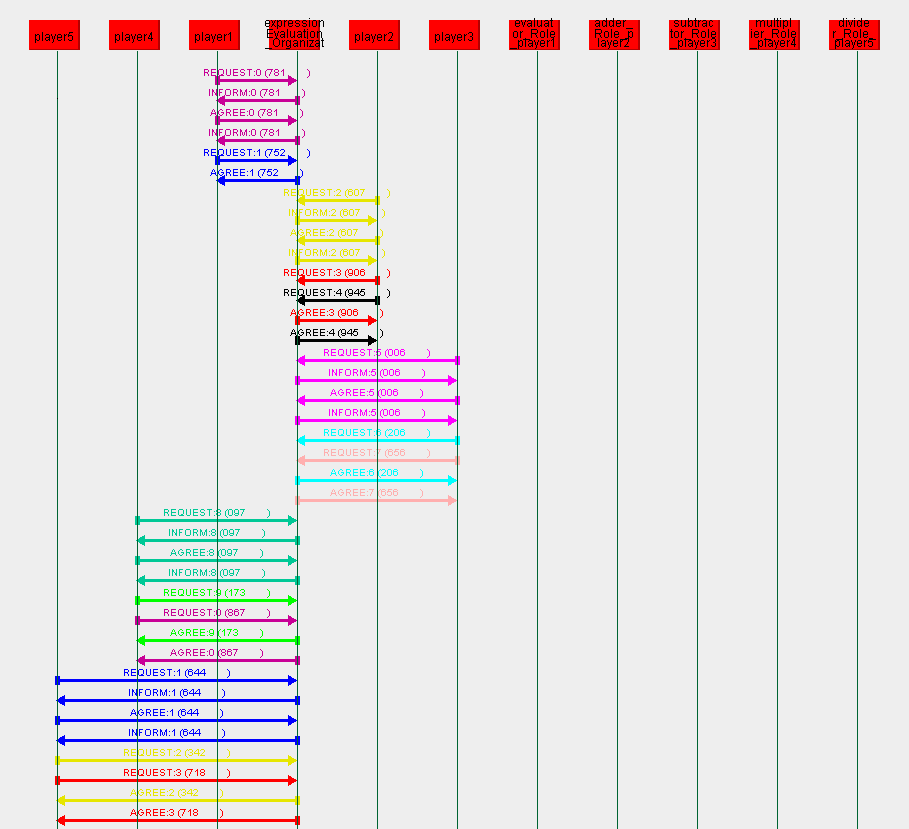
\includegraphics[width=\textwidth]{images/examples/example2-stage1.png}
	\caption{Stage 1: Role enactment}
	\label{figure:example2-stage1}
\end{figure}

% Purple
In the \textbf{purple} interaction scenario, \textit{player1} enacts the \textit{Evaluator} role, resulting in the creation of the \textit{evaluator-player1} position.
% Blue
In the \textbf{blue} interaction scenario, \textit{player1} subscribes to the \textit{Activate role} event.

% First yellow
In the \textbf{first yellow} interaction scenario, \textit{player2} enacts the \textit{Adder} role, resulting in the creation of the \textit{adder-player2} position.
% First red
In the \textbf{first red} interaction scenario, \textit{player2} subscribes to the \textit{Activate role} event.
% Black 
In the \textbf{black} interaction scenario, \textit{player2} subscribes to the \textit{Deactivate role} event.

% Purple
In the \textbf{purple} interaction scenario, \textit{player3} enacts the \textit{Subtractor} role, resulting in the creation of the \textit{subtractor-player3} position.
% Cyan
In the \textbf{cyan} interaction scenario, \textit{player3} subscribes to the \textit{Activate role} event.
% Pink
In the \textbf{pink} interaction scenario, \textit{player3} subscribes to the \textit{Deactivate role} event.

% Dark green
In the \textbf{dark green} interaction scenario, \textit{player4} enacts the \textit{Multiplier} role, resulting in the creation of the \textit{multiplier-player4} position.
% Light green
In the \textbf{light green} interaction scenario, \textit{player4} subscribes to the \textit{Activate role} event.
% Purple
In the \textbf{purple} interaction scenario, \textit{player4} subscribes to the \textit{Deactivate role} event.

% Blue
In the \textbf{blue} interaction scenario, \textit{player5} enacts the \textit{Divider} role, resulting in the creation of the \textit{divider-player5} position.
% Second yellow
In the \textbf{second yellow} interaction scenario, \textit{player5} subscribes to the \textit{Activate role} event.
% Second red
In the \textbf{second red} interaction scenario, \textit{player5} subscribes to the \textit{Deactivate role} event.

%%%%%%%%%%%%%%%%%%%%%%%%%%%%%%%%%%%%%%%%%%%%%%%%%%%%%%%%%%%%%%%%%%%%%%%%%%%%%%%%
\subsubsection*{Stage 2: Role Activation}

% Figure: Stage 2: Role activation
\begin{figure}[H]
	\centering
	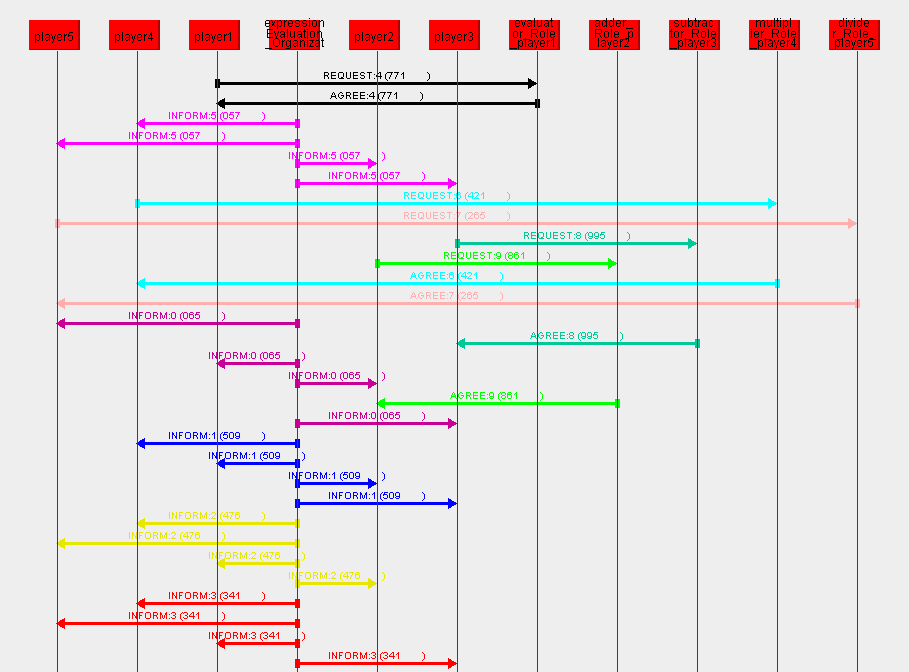
\includegraphics[width=\textwidth]{images/examples/example2-stage2.png}
	\caption{Stage 2: Role activation}
	\label{figure:example2-stage2}
\end{figure}

% Black
In the \textbf{black} interaction scenario, \textit{player1} activates its \textit{Evaluator} role.
% Magenta
In the \textbf{magenta} interaction scenario, the \textit{evaluate-expression} organization publishes the \textit{Role activated} event (for the \textit{Eveluator} role).
\textit{player2} reacts by activating its \textit{Adder} role (the \textbf{light green} interaction scenario), \textit{player3} by activating its \textit{Subtractor} role (the \textbf{dark green} interaction scenario), \textit{player4} by activating its \textit{Multiplier} role (the \textbf{cyan} interaction scenario) and \textit{player5} by activating its \textit{Divider} role (the \textbf{pink} interaction scenario).

% Light green
In the \textbf{light green} interaction scenario, \textit{player2} activates its \textit{Adder} role.
% Red
In the \textbf{blue} interaction scenario, the \textit{evaluate-expression} organization publishes the \textit{Role activated} event (for the \textit{Adder} role).

% Dark green
In the \textbf{dark green} interaction scenario, \textit{player3} activates its \textit{Subtractor} role.
% Yellow
In the \textbf{yellow} interaction scenario, the \textit{evaluate-expression} organization publishes the \textit{Role activated} event (for the \textit{Subtractor} role).

% Cyan
In the \textbf{cyan} interaction scenario, \textit{player4} activates its \textit{Multiplier} role.
% Purple
In the \textbf{purple} interaction scenario, the \textit{evaluate-expression} organization publishes the \textit{Role activated} event (for the \textit{Multiplier} role).

% Pink
In the \textbf{pink} interaction scenario, \textit{player5} activates its \textit{Divider} role.
% Blue
In the \textbf{blue} interaction scenario, the \textit{evaluate-expression} organization publishes the \textit{Role activated} event (for the \textit{Divider} role).

% Event originator not notified
Note that that in all role activation scenarios, the player activating a role is not notified about the resulting \textit{Role activated} event, although it is subscribed to it; there is no need to notify the player causing the event in the first place.

%%%%%%%%%%%%%%%%%%%%%%%%%%%%%%%%%%%%%%%%%%%%%%%%%%%%%%%%%%%%%%%%%%%%%%%%%%%%%%%%
\subsubsection*{Stage 3: Competence and Responsibility Invocation}

The \textit{Evaluate expression} competence is invoked by \textit{player1} from its \textit{Evaluator} role and is carried out in a divide-and-conquer fashion by an \textit{Evaluator}, an \textit{Adder}, a \textit{Multiplier} and a \textit{Divider} by collaborating with one another and invoking responsibilities from their respective players.
In this example the expression to be evaluated is $(1\cdot2)+(4/2)$.

% Evaluator: "(1*2)+(4/2)"
\textit{Evaluator} to evaluate $(1\cdot2)+(4/2)$: it parses the expression and finds the operation to be applied last - addition.
It splits the expression into two sub-expressions and requests \textit{Adder} to evaluate their sum (the \textbf{first magenta} interaction scenario).
It then reports the value (4) to \textit{player1} (the \textbf{first black} interaction scenario).

% Adder: "(1*2)", "(4/2)"
\textit{Adder} to evaluate the sum of $(1\cdot2)$ and $(4/2)$: it requests \textit{Evaluator} to evaluate both expressions (the \textbf{first cyan} and \textbf{blue} interaction scenarios) and invokes the \textit{Add} responsibility on \textit{player2} to calculate the sum of their values (the \textbf{second cyan} interaction scenario).
It then reports the sum (4) to \textit{Evaluator} (the \textit{first magenta} interaction scenario).

% Evaluator: "(1*2)"
\textit{Evaluator} to evaluate $(1\cdot2)$: it parses the expression and finds the last-to-be-applied operation - multiplication.
It splits the expression into two sub-expressions and requests \textit{Multiplier} to evaluate their product (the \textit{pink} interaction scenario).
It then reports the value (2) to \textit{Adder} (the \textbf{first cyan} interaction scenario).

% Multiplier: "1", "2"
\textit{Multiplier} to evaluate the product of $1$ and $2$: it requests \textit{Evaluator} to evaluate both expressions (the \textbf{dark green} and \textbf{light green} interaction scenarios) and invokes the \textit{Multiply} responsibility on \textit{player4} to calculate the product of their values (the \textbf{purple} interaction scenario).
It then reports the product (2) to \textit{Evaluator} (the \textit{pink} interaction scenario).

% Evaluator: "1"
\textit{Evaluator} to evaluate $1$: it parses the expression and finds out it is a number.
It reports the value (1) to \textit{Multiplier} (the \textbf{dark green} interaction scenario).

% Evaluator: "2"
\textit{Evaluator} to evaluate $2$: it parses the expression and finds out it is a number.
It reports the value (2) to \textit{Multiplier} (the \textbf{light green} interaction scenario).

% Evaluator: "(4/2)"
\textit{Evaluator} to evaluate $(1\cdot2)$: it parses the expression and finds the last-to-be-applied operation - division.
It splits the expression into two sub-expressions and requests \textit{Divider} to evaluate their quotient (the \textit{yellow} interaction scenario).
It then reports the value (2) to \textit{Adder} (the \textbf{blue} interaction scenario).

% Divider: "4", "2"
\textit{Divider} to evaluate the quotient of $4$ and $2$: it requests \textit{Evaluator} to evaluate both expressions (the \textbf{red} and \textbf{black} interaction scenarios) and invokes the \textit{Divide} responsibility on \textit{player5} to calculate the quotient of their values (the \textbf{second magenta} interaction scenario).
It then reports the quotient (2) to \textit{Evaluator} (the \textit{yellow} interaction scenario).

% Evaluator: "4"
\textit{Evaluator} to evaluate $4$: it parses the expression and finds out it is a number.
It reports the value (4) to \textit{Divider} (the \textbf{red} interaction scenario).

% Evaluator: "2"
\textit{Evaluator} to evaluate $2$: it parses the expression and finds out it is a number.
It reports the value (2) to \textit{Divider} (the \textbf{black} interaction scenario).

%%%%%%%%%%%%%%%%%%%%%%%%%%%%%%%%%%%%%%%%%%%%%%%%%%%%%%%%%%%%%%%%%%%%%%%%%%%%%%%%
\subsubsection*{Stage 4: Role Deactivation}

% Figure: Stage 4: Role deactivation
\begin{figure}[H]
	\centering
	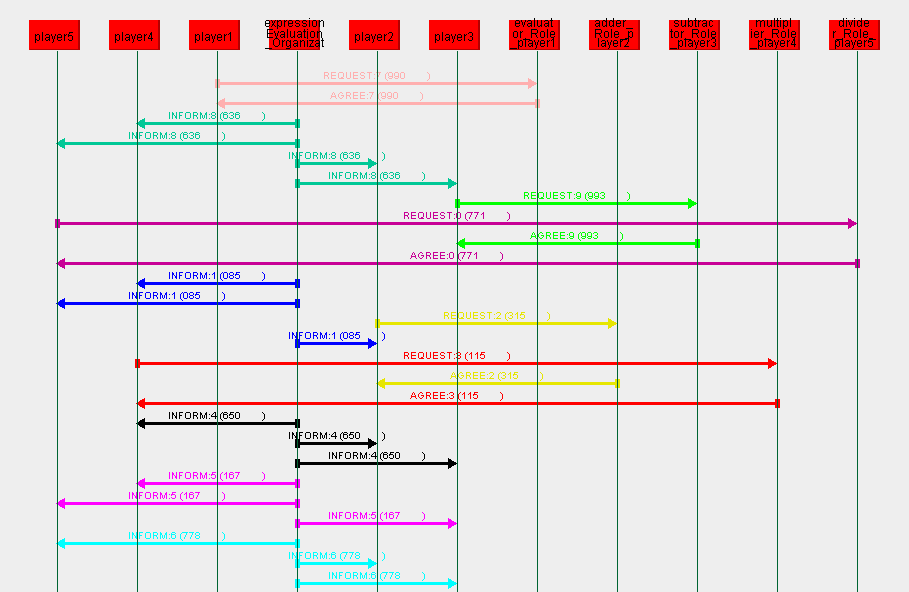
\includegraphics[width=\textwidth]{images/examples/example2-stage4.png}
	\caption{Stage 4: Role deactivation}
	\label{figure:example2-stage4}
\end{figure}

% Pink
In the \textbf{pink} interaction scenario, \textit{player1} deactivates its \textit{Evaluator} role.
% Dark green
In the \textbf{dark green} interaction scenario, the \textit{evaluate-expression} organization publishes the \textit{Role deactivated} event (for the \textit{Eveluator} role).
\textit{player2} reacts by deactivating its \textit{Adder} role (the \textbf{yellow} interaction scenario), \textit{player3} by deactivating its \textit{Subtractor} role (the \textbf{light green} interaction scenario), \textit{player4} by deactivating its \textit{Multiplier} role (the \textbf{red} interaction scenario) and \textit{player5} by deactivating its \textit{Divider} role (the \textbf{purple} interaction scenario).

% Yellow
In the \textbf{yellow} interaction scenario, \textit{player2} deactivates its \textit{Adder} role.
% Magenta
In the \textbf{magenta} interaction scenario, the \textit{evaluate-expression} organization publishes the \textit{Role deactivated} event (for the \textit{Adder} role).

% Light green
In the \textbf{light green} interaction scenario, \textit{player3} deactivates its \textit{Subtractor} role.
% Blue
In the \textbf{blue} interaction scenario, the \textit{evaluate-expression} organization publishes the \textit{Role deactivated} event (for the \textit{Subtractor} role).

% Red
In the \textbf{red} interaction scenario, \textit{player4} deactivates its \textit{Multiplier} role.
% Cyan
In the \textbf{cyan} interaction scenario, the \textit{evaluate-expression} organization publishes the \textit{Role deactivated} event (for the \textit{Multiplier} role).

% Purple
In the \textbf{purple} interaction scenario, \textit{player5} deactivates its \textit{Divider} role.
% Black
In the \textbf{black} interaction scenario, the \textit{evaluate-expression} organization publishes the \textit{Role deactivated} event (for the \textit{Divider} role).

%%%%%%%%%%%%%%%%%%%%%%%%%%%%%%%%%%%%%%%%%%%%%%%%%%%%%%%%%%%%%%%%%%%%%%%%%%%%%%%%
\subsubsection*{Stage 5: Role Deactment}

% Figure: Stage 5: Role deactment
\begin{figure}[H]
	\centering
	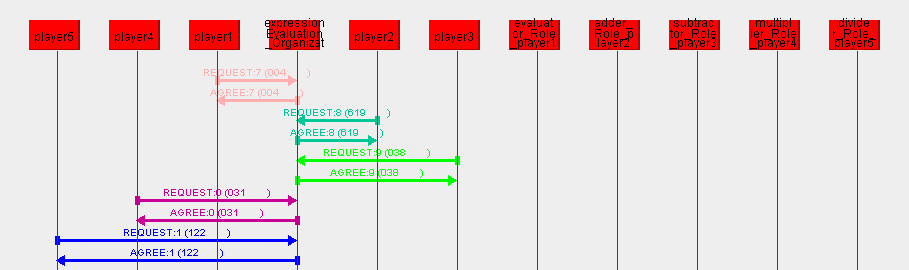
\includegraphics[width=\textwidth]{images/examples/example2-stage5.png}
	\caption{Stage 5: Role deactment}
	\label{figure:example2-stage5}
\end{figure} 

% Pink
In the \textbf{pink} interaction scenario, \textit{player1} deacts its \textit{Evaluator} role.
% Dark green
In the \textbf{dark green} interaction scenario, \textit{player2} deacts its \textit{Adder} role.
% Light green
In the \textbf{light green} interaction scenario, \textit{player3} deacts its \textit{Subtractor} role.
% Purple
In the \textbf{purple} interaction scenario, \textit{player4} deacts its \textit{Multiplier} role.
% Blue
In the \textbf{blue} interaction scenario, \textit{player5} deacts its \textit{Divider} role.